\documentclass[specialist,
			   substylefile = spbu_report.rtx,
			   subf,href,colorlinks=true, 12pt]{disser}

\usepackage[a4paper,
			mag=1000, includefoot,
			left=3cm, right=1.5cm, top=2cm, bottom=2cm, headsep=1cm, footskip=1cm]{geometry}
\usepackage[utf8]{inputenc}
\usepackage[backend = bibtex8,sorting=none]{biblatex}
\usepackage[T2A]{fontenc}
\usepackage[english,russian]{babel}
\usepackage{amsfonts}
\usepackage{amssymb}
\usepackage{amsmath}
\usepackage{listings}
\usepackage{graphicx}
\usepackage{tabularx}
\usepackage{float}
\usepackage{slashbox}
\usepackage{xcolor}
%new calligraphic font for subspaces
\usepackage{euscript}
\newcommand{\cA}{\EuScript{A}}
\newcommand{\cB}{\EuScript{B}}
\newcommand{\cC}{\EuScript{C}}
\newcommand{\cD}{\EuScript{D}}
\newcommand{\cE}{\EuScript{E}}
\newcommand{\cF}{\EuScript{F}}
\newcommand{\cG}{\EuScript{G}}
\newcommand{\cH}{\EuScript{H}}
\newcommand{\cI}{\EuScript{I}}
\newcommand{\cJ}{\EuScript{J}}
\newcommand{\cK}{\EuScript{K}}
\newcommand{\cL}{\EuScript{L}}
\newcommand{\cM}{\EuScript{M}}
\newcommand{\cN}{\EuScript{N}}
\newcommand{\cO}{\EuScript{O}}
\newcommand{\cP}{\EuScript{P}}
\newcommand{\cQ}{\EuScript{Q}}
\newcommand{\cR}{\EuScript{R}}
\newcommand{\cS}{\EuScript{S}}
\newcommand{\cT}{\EuScript{T}}
\newcommand{\cU}{\EuScript{U}}
\newcommand{\cV}{\EuScript{V}}
\newcommand{\cW}{\EuScript{W}}
\newcommand{\cX}{\EuScript{X}}
\newcommand{\cY}{\EuScript{Y}}
\newcommand{\cZ}{\EuScript{Z}}

%font for text indices like transposition X^\mathrm{T}
\newcommand{\rmA}{\mathrm{A}}
\newcommand{\rmB}{\mathrm{B}}
\newcommand{\rmC}{\mathrm{C}}
\newcommand{\rmD}{\mathrm{D}}
\newcommand{\rmE}{\mathrm{E}}
\newcommand{\rmF}{\mathrm{F}}
\newcommand{\rmG}{\mathrm{G}}
\newcommand{\rmH}{\mathrm{H}}
\newcommand{\rmI}{\mathrm{I}}
\newcommand{\rmJ}{\mathrm{J}}
\newcommand{\rmK}{\mathrm{K}}
\newcommand{\rmL}{\mathrm{L}}
\newcommand{\rmM}{\mathrm{M}}
\newcommand{\rmN}{\mathrm{N}}
\newcommand{\rmO}{\mathrm{O}}
\newcommand{\rmP}{\mathrm{P}}
\newcommand{\rmQ}{\mathrm{Q}}
\newcommand{\rmR}{\mathrm{R}}
\newcommand{\rmS}{\mathrm{S}}
\newcommand{\rmT}{\mathrm{T}}
\newcommand{\rmU}{\mathrm{U}}
\newcommand{\rmV}{\mathrm{V}}
\newcommand{\rmW}{\mathrm{W}}
\newcommand{\rmX}{\mathrm{X}}
\newcommand{\rmY}{\mathrm{Y}}
\newcommand{\rmZ}{\mathrm{Z}}

%tt font for time series
\newcommand{\tA}{\mathbb{A}}
\newcommand{\tB}{\mathbb{B}}
\newcommand{\tC}{\mathbb{C}}
\newcommand{\tD}{\mathbb{D}}
\newcommand{\tE}{\mathbb{E}}
\newcommand{\tF}{\mathbb{F}}
\newcommand{\tG}{\mathbb{G}}
\newcommand{\tH}{\mathbb{H}}
\newcommand{\tI}{\mathbb{I}}
\newcommand{\tJ}{\mathbb{J}}
\newcommand{\tK}{\mathbb{K}}
\newcommand{\tL}{\mathbb{L}}
\newcommand{\tM}{\mathbb{M}}
\newcommand{\tN}{\mathbb{N}}
\newcommand{\tO}{\mathbb{O}}
\newcommand{\tP}{\mathbb{P}}
\newcommand{\tQ}{\mathbb{Q}}
\newcommand{\tR}{\mathbb{R}}
\newcommand{\tS}{\mathbb{S}}
\newcommand{\tT}{\mathbb{T}}
\newcommand{\tU}{\mathbb{U}}
\newcommand{\tV}{\mathbb{V}}
\newcommand{\tW}{\mathbb{W}}
\newcommand{\tX}{\mathbb{X}}
\newcommand{\tY}{\mathbb{Y}}
\newcommand{\tZ}{\mathbb{Z}}

%bf font for matrices
\newcommand{\bfA}{\mathbf{A}}
\newcommand{\bfB}{\mathbf{B}}
\newcommand{\bfC}{\mathbf{C}}
\newcommand{\bfD}{\mathbf{D}}
\newcommand{\bfE}{\mathbf{E}}
\newcommand{\bfF}{\mathbf{F}}
\newcommand{\bfG}{\mathbf{G}}
\newcommand{\bfH}{\mathbf{H}}
\newcommand{\bfI}{\mathbf{I}}
\newcommand{\bfJ}{\mathbf{J}}
\newcommand{\bfK}{\mathbf{K}}
\newcommand{\bfL}{\mathbf{L}}
\newcommand{\bfM}{\mathbf{M}}
\newcommand{\bfN}{\mathbf{N}}
\newcommand{\bfO}{\mathbf{O}}
\newcommand{\bfP}{\mathbf{P}}
\newcommand{\bfQ}{\mathbf{Q}}
\newcommand{\bfR}{\mathbf{R}}
\newcommand{\bfS}{\mathbf{S}}
\newcommand{\bfT}{\mathbf{T}}
\newcommand{\bfU}{\mathbf{U}}
\newcommand{\bfV}{\mathbf{V}}
\newcommand{\bfW}{\mathbf{W}}
\newcommand{\bfX}{\mathbf{X}}
\newcommand{\bfY}{\mathbf{Y}}
\newcommand{\bfZ}{\mathbf{Z}}

%bb font for standard spaces and expectation
\newcommand{\bbA}{\mathbb{A}}
\newcommand{\bbB}{\mathbb{B}}
\newcommand{\bbC}{\mathbb{C}}
\newcommand{\bbD}{\mathbb{D}}
\newcommand{\bbE}{\mathbb{E}}
\newcommand{\bbF}{\mathbb{F}}
\newcommand{\bbG}{\mathbb{G}}
\newcommand{\bbH}{\mathbb{H}}
\newcommand{\bbI}{\mathbb{I}}
\newcommand{\bbJ}{\mathbb{J}}
\newcommand{\bbK}{\mathbb{K}}
\newcommand{\bbL}{\mathbb{L}}
\newcommand{\bbM}{\mathbb{M}}
\newcommand{\bbN}{\mathbb{N}}
\newcommand{\bbO}{\mathbb{O}}
\newcommand{\bbP}{\mathbb{P}}
\newcommand{\bbQ}{\mathbb{Q}}
\newcommand{\bbR}{\mathbb{R}}
\newcommand{\bbS}{\mathbb{S}}
\newcommand{\bbT}{\mathbb{T}}
\newcommand{\bbU}{\mathbb{U}}
\newcommand{\bbV}{\mathbb{V}}
\newcommand{\bbW}{\mathbb{W}}
\newcommand{\bbX}{\mathbb{X}}
\newcommand{\bbY}{\mathbb{Y}}
\newcommand{\bbZ}{\mathbb{Z}}

%got font for any case
\newcommand{\gA}{\mathfrak{A}}
\newcommand{\gB}{\mathfrak{B}}
\newcommand{\gC}{\mathfrak{C}}
\newcommand{\gD}{\mathfrak{D}}
\newcommand{\gE}{\mathfrak{E}}
\newcommand{\gF}{\mathfrak{F}}
\newcommand{\gG}{\mathfrak{G}}
\newcommand{\gH}{\mathfrak{H}}
\newcommand{\gI}{\mathfrak{I}}
\newcommand{\gJ}{\mathfrak{J}}
\newcommand{\gK}{\mathfrak{K}}
\newcommand{\gL}{\mathfrak{L}}
\newcommand{\gM}{\mathfrak{M}}
\newcommand{\gN}{\mathfrak{N}}
\newcommand{\gO}{\mathfrak{O}}
\newcommand{\gP}{\mathfrak{P}}
\newcommand{\gQ}{\mathfrak{Q}}
\newcommand{\gR}{\mathfrak{R}}
\newcommand{\gS}{\mathfrak{S}}
\newcommand{\gT}{\mathfrak{T}}
\newcommand{\gU}{\mathfrak{U}}
\newcommand{\gV}{\mathfrak{V}}
\newcommand{\gW}{\mathfrak{W}}
\newcommand{\gX}{\mathfrak{X}}
\newcommand{\gY}{\mathfrak{Y}}
\newcommand{\gZ}{\mathfrak{Z}}

%old calligraphic font
\newcommand{\calA}{\mathcal{A}}
\newcommand{\calB}{\mathcal{B}}
\newcommand{\calC}{\mathcal{C}}
\newcommand{\calD}{\mathcal{D}}
\newcommand{\calE}{\mathcal{E}}
\newcommand{\calF}{\mathcal{F}}
\newcommand{\calG}{\mathcal{G}}
\newcommand{\calH}{\mathcal{H}}
\newcommand{\calI}{\mathcal{I}}
\newcommand{\calJ}{\mathcal{J}}
\newcommand{\calK}{\mathcal{K}}
\newcommand{\calL}{\mathcal{L}}
\newcommand{\calM}{\mathcal{M}}
\newcommand{\calN}{\mathcal{N}}
\newcommand{\calO}{\mathcal{O}}
\newcommand{\calP}{\mathcal{P}}
\newcommand{\calQ}{\mathcal{Q}}
\newcommand{\calR}{\mathcal{R}}
\newcommand{\calS}{\mathcal{S}}
\newcommand{\calT}{\mathcal{T}}
\newcommand{\calU}{\mathcal{U}}
\newcommand{\calV}{\mathcal{V}}
\newcommand{\calW}{\mathcal{W}}
\newcommand{\calX}{\mathcal{X}}
\newcommand{\calY}{\mathcal{Y}}
\newcommand{\calZ}{\mathcal{Z}}

\newcommand{\bt}{\begin{theorem}}
\newcommand{\et}{\end{theorem}}
\newcommand{\bl}{\begin{lemma}}
\newcommand{\el}{\end{lemma}}
\newcommand{\bp}{\begin{proposition}}
\newcommand{\ep}{\end{proposition}}
\newcommand{\bc}{\begin{corollary}}
\newcommand{\ec}{\end{corollary}}

\newcommand{\bd}{\begin{definition}\rm}
\newcommand{\ed}{\end{definition}}
\newcommand{\bex}{\begin{example}\rm}
\newcommand{\eex}{\end{example}}
\newcommand{\br}{\begin{remark}\rm}
\newcommand{\er}{\end{remark}}

\newcommand{\btbh}{\begin{table}[!ht]}
\newcommand{\etb}{\end{table}}
\newcommand{\bfgh}{\begin{figure}[!ht]}
\newcommand{\efg}{\end{figure}}

\newcommand{\bea}{\begin{eqnarray*}}
\newcommand{\eea}{\end{eqnarray*}}
\newcommand{\be}{\begin{eqnarray}}
\newcommand{\ee}{\end{eqnarray}}
%
\newcommand{\intl}{\int\limits}
\newcommand{\suml}{\sum\limits}
\newcommand{\liml}{\lim\limits}
\newcommand{\prodl}{\prod\limits}
\newcommand{\minl}{\min\limits}
\newcommand{\maxl}{\max\limits}
\newcommand{\supl}{\sup\limits}
%
\newcommand{\ve}{\varepsilon}
\newcommand{\vphi}{\varphi}
\newcommand{\ovl}{\overline}
\newcommand{\lm}{\lambda}
\def\wtilde{\widetilde}
\def\what{\widehat}

\newcommand{\ra}{\rightarrow}
\newcommand{\towith}[1]{\mathrel{\mathop{\longrightarrow}_{#1}}}

\def\bproof{\textbf{Proof.\ }}
\def\eproof{\hfill$\Box$\smallskip}

\def\spaceR{\mathsf{R}}
\def\spaceC{\mathsf{C}} %is not used?
\newcommand\Expect{\mathsf{E}}


\newcommand{\bfw}{\mathbf{w}}

\def\last#1{{\underline{#1}}}
\def\first#1{{\mathstrut\overline{#1}}}
\def\overo#1{\overset{_\mathrm{o}}{#1}}
\newcommand{\ontop}[2]{\genfrac{}{}{0pt}{0}{#1}{#2}}

\def\sspan{\mathop{\mathrm{span}}}
\def\rank{\mathop{\mathrm{rank}}}
\def\dist{\mathop{\mathrm{dist}}}
\newcommand{\diag}{\mathop{\mathrm{diag}}}
\newcommand{\reverse}{\mathop{\mathrm{rev}}}
\newcommand{\Arg}{\mathop\mathrm{Arg}}
\newcommand{\meas}{\mathop{\mathrm{meas}}}

\makeatletter
\def\adots{\mathinner{\mkern2mu\raise\p@\hbox{.}
\mkern2mu\raise4\p@\hbox{.}\mkern1mu
\raise7\p@\vbox{\kern7\p@\hbox{.}}\mkern1mu}}
\newcommand{\l@abcd}[2]{\hbox to\textwidth{#1\dotfill #2}}
\makeatother

\ifpdf\usepackage{epstopdf}\fi
% Точка с запятой в качестве разделителя между номерами цитирований
%\setcitestyle{semicolon}

% Добавить больший абзац после листинга
\lstset{
	belowskip=20pt,
	showstringspaces=false
}

% форматирование языка RsT
\lstdefinelanguage{RsT}
{
	directives={example, Example, EXAMPLE},
	delim=*[directive]{..\ },
	directivestyle=\color{red}\underbar,
}[
keywords,
directives,
comments,
]

\graphicspath{ {images/} }
\addbibresource{lit.bib}

% Использовать полужирное начертание для векторов
\let\vec=\mathbf

% Включать подсекции в оглавление
\setcounter{tocdepth}{2}

\makeatletter
\setlength{\@fptop}{0pt}
\makeatother

%----------------------------------------------------------------
\begin{document}

%
% Титульный лист на русском языке
%
% Название организации
\institution{%
	Санкт-Петербургский государственный университет\\
	Прикладная математика и информатика
}

\title{Отчет по производственной практике (педагогической) (семестр 3)}

% Тема
\topic{Написание файла помощи для SSA на Python}

% Автор
\author{Козак Михаил Валерьевич}
\group{группа 21.М03-мм}

% Научный руководитель
\sa       {Голяндина Нина Эдуардовна\\%
		   Кафедра Статистического Моделирования}
\sastatus {к.\,ф.-м.\,н., доцент}

% Город и год
\city{Санкт-Петербург}
\date{2022}

\maketitle

\tableofcontents

\chapter{Введение}

Singular spectrum analysis (SSA) \cite{ssa-method} – метод для анализа временных рядов, основанный на преобразовании одномерного временного ряда в многомерный, с последующим применением к нему метода главных компонент. Данный метод находит применение в различных сферах: климатология, океанология, геофизика, техника, обработка изображений, медицина, эконометрика и многие другие. \\

Данный метод активно применяется в обучении студентов, в связи с чем требуется своевременная адаптация инструментов, позволяющих применять его на практике. С этой целью для использования метода SSA в популярном языке программирования Python ведется разработка пакета pyrssa \cite{pyrssa-lib}, который является адаптацией существующей для языка R библиотеки Rssa \cite{rssa-book, rssa-doc}, использующей алгоритмы, реализованные на языке C с целью повышения скорости работы. 

Пакет Rssa  содержит исчерпывающую документацию, в которой есть как информация по самим функциям библиотеки и примерам их использования, так и ссылки на литературу с описанием алгоритмов, которые легли в основу пакета. Вся эта информация позволяет обучающимся достаточно быстро получать справку и о методах, и об инструментах для их применения. Необходимость переноса существующей документации вызвана в первую очередь тем, что адаптированная для Python версия пакета в силу отличий от языка R содержит изменения как в структуре модулей, так и в доступных и используемых типах данных. В силу отличий синтаксиса языков возникла необходимость произвести адаптацию примеров использования пакета  для документации, а также для удобства обучающихся: вся необходимая информация должна быть доступна пользователям сразу и в наглядном формате.

Таким образом, в рамках данной работы стояла задача создания и оформления файлов помощи для пакета pyrssa, основываясь на уже существующей документации для Rssa. 

Помимо непосредственно адаптации также стояла задача максимально упростить для пользователей взаимодействие с документацией – предоставить различные способы обращения к ней, а также создать удобную структуру и возможность навигации по файлам помощи. Наиболее универсальным способом на текущий момент являются веб-страницы, в связи с тем, что они адаптированы для различных устройств, будь то стационарные компьютеры или мобильные устройства, а также для различных операционных систем. В связи с этим главной задачей являлось написание документации в формате веб-сайта и его публикация в интернете для общего доступа.


\chapter{Документация для pyrssa}

Для оформления документации был выбран пакет sphinx \cite{sphinx-lib}, обладающий обширной функциональностью и, что самое главное, достаточно высоким уровнем автоматизации работы: определение структуры модуля, к которому пишется документация, создание удобных заготовок веб-страниц с навигацией, простое, но многофункциональное форматирование текста документации, связывание ссылок на определенные в модуле классы – лишь часть доступных возможностей. Во многом благодаря этому данный пакет стал стандартом для оформления документации библиотек, написанных на языке Python. Далее будут описаны предпринятые для создания файлов помощи действия.

\section{Создание заготовок для веб-страниц}

В первую очередь, после установки самого пакета, требуется выполнить набор простых команд в терминале для создания заготовки файла конфигурации, который содержит основную информацию о библиотеке, такую как название и автор, а также позволяет выбрать используемые расширения, позволяющие ускорить работу с документацией, указать директории, в которых будет производиться поиск при создании веб-страниц, и исключить те, которые не должны приниматься в рассмотрение. Ниже приведено примерное содержание данного файла за исключением комментариев, которые создаются для навигации в случае возникновения вопросов при оформлении.

\begin{lstlisting}[language=Python, caption=Содержимое конфигурационного файла.]
	
	from sphinx.ext import autodoc
	import os
	import sys
	sys.path.insert(0, os.path.abspath('..'))

	project = 'pyrssa'
	copyright = '2023, Fleyderer'
	author = 'Fleyderer'
	release = '1.0.6'
	
	extensions = [
	'sphinx.ext.autodoc',
	'sphinx.ext.viewcode',
	'sphinx.ext.napoleon'
	]
	
	templates_path = ['_templates']
	exclude_patterns = ['_build', 'Thumbs.db', '.DS_Store']
	
	html_theme = 'sphinx_rtd_theme'
	html_static_path = ['_static']
	add_module_names = False
	
	class MockedClassDocumenter(autodoc.ClassDocumenter):
	def add_line(self,
	             line: str, 
	             source: str, *lineno: int) -> None:
	if line == "   Bases: :py:class:`object`":
	return
	super().add_line(line, source, *lineno)
	
	autodoc.ClassDocumenter = MockedClassDocumenter
\end{lstlisting}

В указанном выше фрагменте кода импортируются необходимые модули, указывается основная директория для поиска при сборке HTML-файлов, а также информация о пакете, выбираются необходимые расширения, которые проводят автоматический парсинг написанной документации в соответствии с различными стилями форматирования текста. Помимо этого указываются исключаемые файлы, устанавливается визуальный стиль оформления веб-страниц, а также создается дополнительная обертка для того, чтобы исключать из генерируемых файлов ненужную информацию, которая не понадобится пользователю. Наполнение этой обертки остается на усмотрение пользователя.

После того, как данный файл успешно оформлен, необходимо сгенерировать файлы с расширением .rst – это расширение файлов типа reStructuredText \cite{rst-doc}, являющегося облегчённым языком разметки. С помощью таких файлов оформление навигации становится проще, чем при использовании стандартного HTML. Для этого терминал открывается в основной директории модуля и при выполнении команды для создания файлов выбирается дочерняя директория, внутри которой эти файлы должны находиться. После этого, если при выполнении предыдущих действий не были допущены ошибки, создаются файлы разметки. Во фрагменте кода, приведенном ниже, указано примерное содержание заглавной страницы документации, написанной с помощью reStructureText.

\begin{lstlisting}[language=RsT, caption=Содержимое файла заглавной страницы документации.]
	Welcome to pyrssa's documentation!
	==================================
	
	Methods and tools for Singular Spectrum Analysis
	in Python...

	
	.. toctree::
	:maxdepth: 2
	:caption: Contents:
	
	pyrssa
	
	
	Indices and tables
	==================
	
	* :ref:`genindex`
	* :ref:`modindex`
	* :ref:`search`
\end{lstlisting}
	
После внесения необходимых правок в относящиеся к модулю .rst-файлы, будь то изменения в структуре документации или же наполнении отдельных страниц, с помощью простой команды создаются файлы HTML, которые доступны для просмотра на различных устройствах. Примерный внешний вид заглавной веб-страницы приведен на иллюстрациях ниже.

\begin{figure}[H]
	\centering
	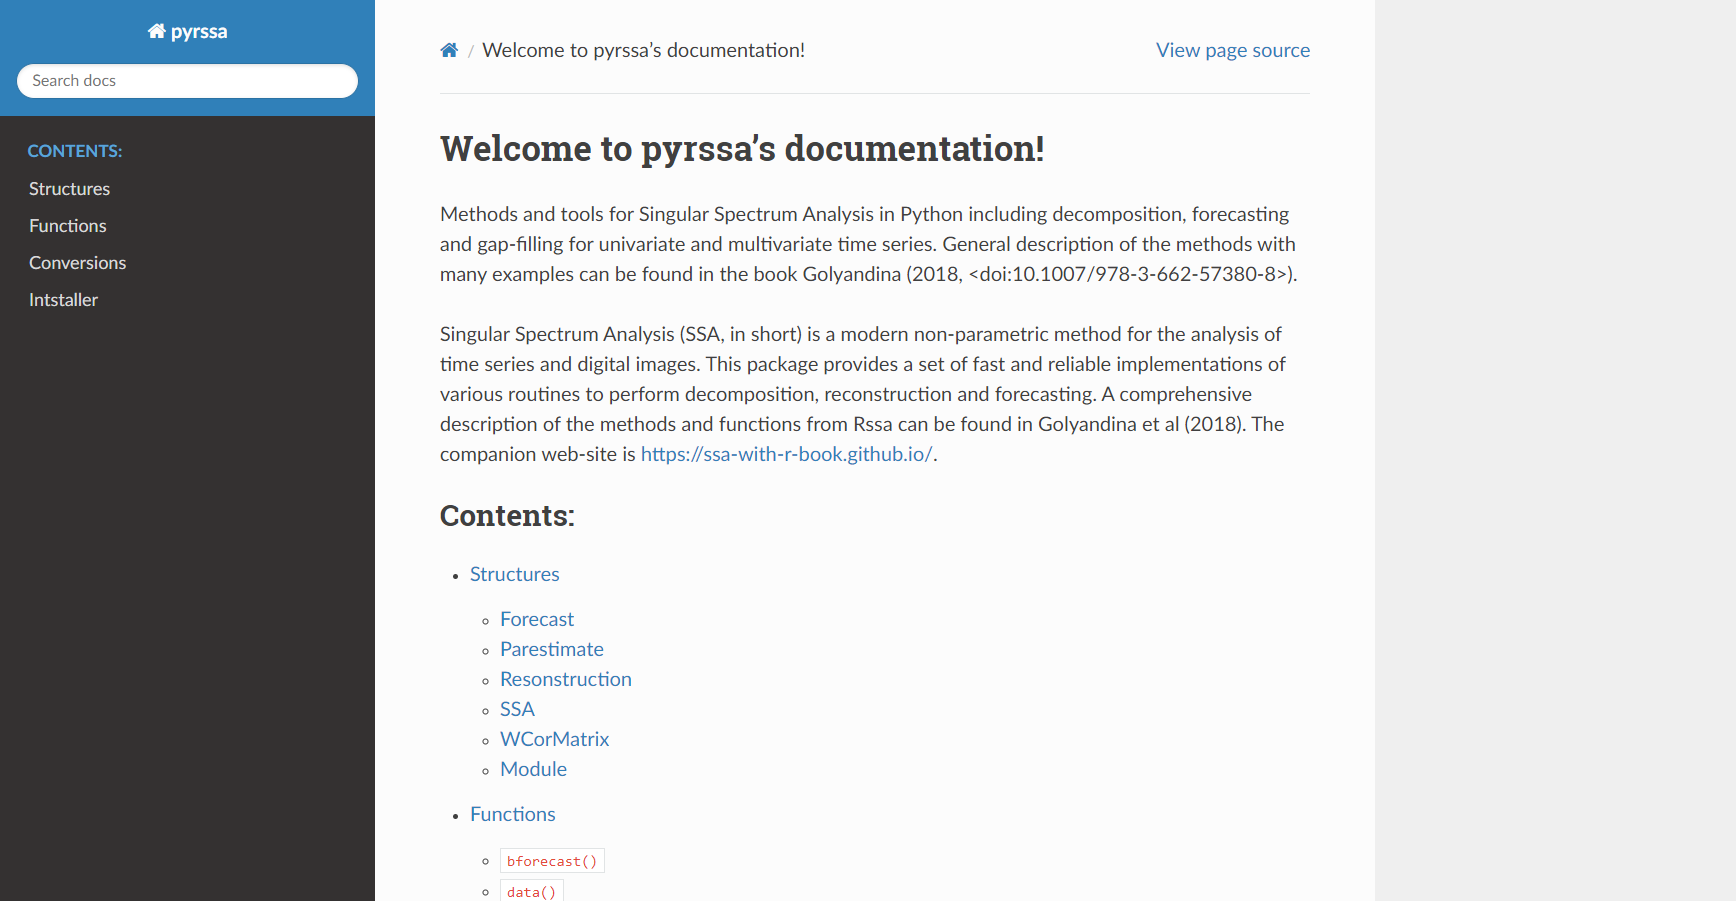
\includegraphics[width=0.8\textwidth]{index_page_pc}
	\caption{Внешний вид страницы для стационарных устройств.}
	\label{fig:index_page_pc}
\end{figure}

\begin{figure}[H]
	\centering
	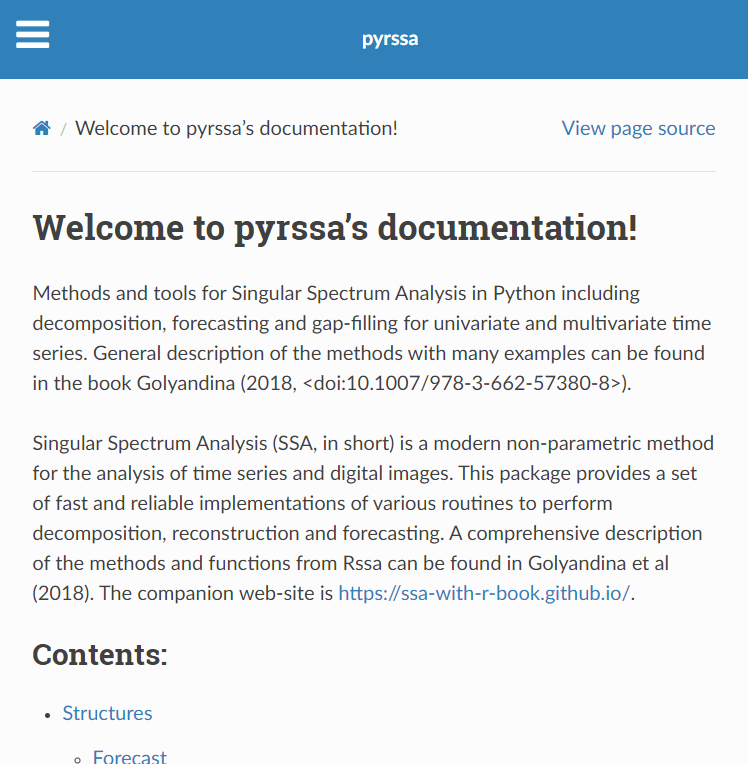
\includegraphics[width=0.6\textwidth]{index_page_mobile}
	\caption{Внешний вид страницы для мобильных устройств.}
	\label{fig:index_page_mobile}
\end{figure}

\section{Написание документации}

После описания структуры документации и создания заглавной страницы необходимо наполнить документацию. Для описания параметров функций, подробной информации, примеров использования и замечаний в Python создаются так называемые docstrings \cite{docstring-doc} – строковые переменные, которые указываются сразу после объявления объектов в языке – таким образом и происходит описание функций в языке Python. Структура возможной строки будет приведена в листинге ниже.

\begin{lstlisting}[language=RsT, caption=Сокращенное содержание docstring для функции reconstruct.]
	:param x: SSA object
	:type x: SSA
	...
	
	Description
	===========
	
	Reconstruct the data given the SSA decomposition and 
	the desired grouping of the elementary components.
	
	Details
	=======
	
	Reconstruction is performed in a common form for 
	different types of input objects
	...
	
	Note
	----
	
	By default (argument drop.attributes) the routine tries 
	to preserve all the attributes of the input object
	...
	
	References
	----------
	
	Golyandina N., Korobeynikov A., Zhigljavsky A. (2018): 
	Singular Spectrum Analysis with R. Use R!. Springer,
	Berlin, Heidelberg
	...
	
	Examples
	--------
	
	.. code-block:: python
	...
\end{lstlisting}

Когда строка информации создана, пользователь может получить информацию о работе функций либо с помощью встроенной в Python функции help(), либо, при использовании продвинутых сред программирования, наведя курсор на функцию, получить информацию в отформатированном виде.

При повторной генерации HTML-файлов веб-страниц, строки документации также учитываются и сопоставляются с функциями модуля внутри файлов помощи, подхватывая форматирование на языке reStructuredText. Результат для функции reconstruct приведен на иллюстрациях ниже.

\begin{figure}[H]
	\centering
	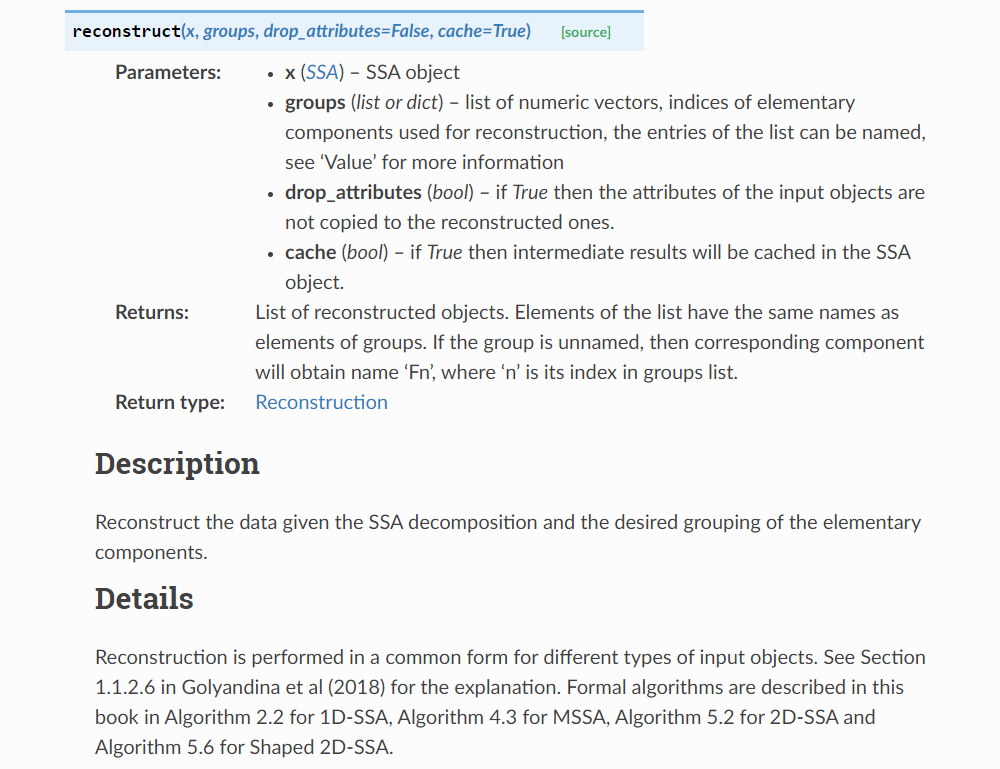
\includegraphics[width=0.8\textwidth]{rec_par}
	\caption{Внешний вид документации для параметров и описания функции reconstruct.}
	\label{fig:rec_par}
\end{figure}

\begin{figure}[H]
	\centering
	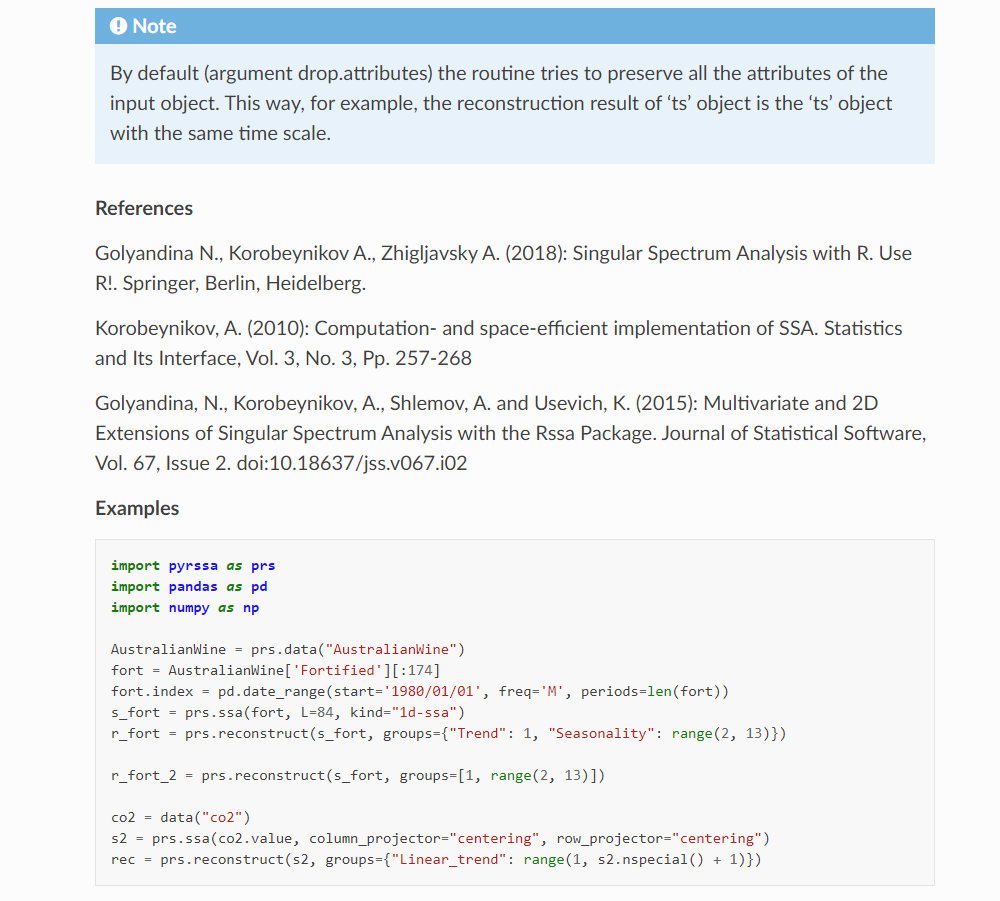
\includegraphics[width=0.6\textwidth]{rec_examples}
	\caption{Внешний вид для замечаний и примеров функции reconstruct.}
	\label{fig:rec_examples}
\end{figure}

\section{Публикация сайта}

Для публикации сайта был выбран хостинг Github Pages \cite{pages-site}, который позволяет опубликовать документацию для общего доступа на основе репозитория, в котором хранится сам пакет pyrssa. Для решения данной задачи необходимо лишь провести предварительную настройку источника загрузки для файлов, относящихся к сайту, и немного изменить структуру их хранения, чтобы Github мог их распознать. Ключевым фактором является наличие в корневой папке файла index.html, который и будет выдавать хостинг при переходе по ссылке. По умолчанию при создании HTML-файлов они находятся во внутренних папках, поэтому сперва проводится корректировка файлов генерации с указанием нужных директорий, а также в корневой папке документации создается небольшой файл index.html, который переадресует на действительную заглавную страницу сайта.

\begin{lstlisting}[language=HTML, caption=Содержимое переадресующего файла index.html.]
	
	<!DOCTYPE html>
	<html lang="en">
	<meta http-equiv="refresh" content="0;
	 url=./html/index.html" />
	</html>
	
\end{lstlisting}

После проведения указанных действий Github при каждом обновлении репозитория, а если быть точнее, ветки, из которой должна подгружаться документация, автоматически их обновляет и спустя пару минут обновленное наполнение сайта становится доступным пользователям.

\chapter{Заключение}

В рамках данной работы были успешно адаптированы файлы помощи пакета Rssa для основных реализованных в pyrssa функций и структур данных, состоящие из их описания, подробной информации и примеров использования в языке Python.

Для достижения этой цели были адаптированы тексты документации Rssa с учетом особенностей реализации на языке Python, к которым относятся типы данных и структуры объектов. Также для большей наглядности были адаптированы и приведены в документации примеры использования функций пакета pyrssa. 

С учетом задачи повышения удобства взаимодействия обучающихся с документацией, помимо адаптации существующих текстов и примеров выполнена работа по написанию документации в формате веб-сайта, содержащего как саму документацию, так и навигацию по страницам. 

Данный веб-сайт опубликован в общем доступе \cite{pyrrsa-doc}, в связи с чем обучающиеся и пользователи могут быстро получить необходимую справку не только внутри используемой среды программирования, но также и при поиске информации в интернете.

\printbibliography
\addcontentsline{toc}{chapter}{Список литературы}

\end{document}